%==============================================================================
%  Beating a Published Baseline on GastroVision
%  Academic-paper rewrite of report/BAO_CAO.md (AIN501 final project).
%
%  Compile: pdflatex paper.tex  (x2 for references)  --- or upload to Overleaf.
%  Uses only standard packages (article, graphicx, booktabs, amsmath, hyperref).
%==============================================================================
\documentclass[11pt,a4paper]{article}

\usepackage[T1]{fontenc}
\usepackage[utf8]{inputenc}
\usepackage{newtxtext,newtxmath}     % Times-like text + math (JCSC look)
\usepackage[margin=2.4cm]{geometry}
\usepackage{graphicx}
\usepackage{booktabs}
\usepackage{amsmath}
\usepackage{array}
\usepackage{multirow}
\usepackage{caption}
\usepackage{siunitx}
\usepackage[hidelinks]{hyperref}
\usepackage{xcolor}
\usepackage{authblk}

\setlength{\emergencystretch}{3em}   % avoid overfull boxes from unbreakable math/names
\captionsetup{font=small,labelfont=bf,justification=centering}
\captionsetup[table]{skip=4pt}
\renewcommand{\arraystretch}{1.12}
\setlength{\parindent}{1.4em}

% Compact section titles, small-caps flavour close to the reference journal.
\usepackage{titlesec}
\titleformat{\section}{\normalfont\large\bfseries\scshape}{\thesection.}{0.6em}{}
\titleformat{\subsection}{\normalfont\normalsize\bfseries}{\thesubsection.}{0.5em}{}

\newcommand{\macroF}{\textup{macro-F1}}   % robust in text and math mode

%------------------------------------------------------------------------------
\title{\vspace{-1.0cm}\bfseries\Large A Measurement-First Study of CNN, Transformer,
and Hybrid Models for 22-Class Gastrointestinal Endoscopy Classification:
Where a $+0.09$ Macro-F1 Gain over the Published Baseline Actually Comes From}

\author{Ho Khac Bac}
\author{Le Trong Quang}
\affil{\normalsize AIN501 --- Artificial Intelligence (Deep Learning), MSE, FPT School of Business \& Technology}
\date{August 31, 2026}

%------------------------------------------------------------------------------
\begin{document}
\maketitle

\begin{abstract}
\noindent\textbf{Abstract.}
The GastroVision benchmark (arXiv:2307.08140, Table~2) reports a \macroF{} of
\textbf{0.6504} for a fully fine-tuned DenseNet-121 on 22 classes / 7{,}930
gastrointestinal (GI) endoscopy images. We do two things and keep them
separate. First, we reproduce the baseline: under the paper's own protocol
(single best-by-validation checkpoint, no test-time augmentation) our
DenseNet-121 reaches $0.6686\pm0.0234$ over three seeds --- $+0.0182$, i.e.
$0.78\sigma$, in 30 epochs rather than 150. Second, we beat it: our proposed
system --- \emph{CoAtNet-0 @288 + a modern training recipe + a top-3 checkpoint
ensemble + inference-time logit adjustment} --- reaches a \macroF{} of
$\mathbf{0.7441\pm0.0088}$, i.e. $+0.0937$, with a bootstrap 95\% confidence
interval of $[0.6986,\,0.7736]$ that \emph{excludes} 0.6504.
The central result, however, is not the number but its decomposition. When the
whole gain is split into independently measured levers under one scoring rule,
the two levers we designed the study to test --- \emph{swapping the
architecture} ($+0.0034$) and \emph{raising the input resolution}
($+0.0041$) --- are indistinguishable from zero. What pays is the
\emph{training recipe} ($+0.0443$) and the \emph{measurement discipline}
(checkpoint rule $+0.0094$, logit adjustment $+0.0143$, at zero extra training
epochs). Yet even the recipe is not universal: the same recipe applied to
DenseNet-121 gives $-0.0110$ (3/3 seeds negative). A completed $2{\times}2$
design isolates the true term as an \emph{interaction} between recipe and
architecture ($+0.0468$), not a sum of two levers. On a dataset with a
$50.6\times$ class imbalance and two classes holding fewer than ten test
images, the bootstrap CI is $\pm0.035$ wide --- larger than four of our five
levers --- so much of the real engineering is variance reduction, and most
textbook long-tail levers applied \emph{at training time} are flat.
All numbers in this paper are extracted automatically from saved notebook
outputs or recomputed from stored logits; none are typed by hand.

\smallskip
\noindent\textbf{Keywords.} medical image classification, gastrointestinal
endoscopy, class imbalance, convolutional networks, vision transformers, hybrid
architectures, reproducibility, macro-F1.
\end{abstract}

%==============================================================================
\section{Introduction}
%==============================================================================

Deep models for medical imaging are usually reported as a single headline
number: one architecture, one run, one metric. Two properties of small,
long-tailed medical datasets make that reporting style fragile. First, the
evaluation set is small and heavily imbalanced, so the run-to-run noise of a
single measurement can exceed the effect one wants to claim. Second, published
baselines are themselves single runs without error bars, so ``we beat the
baseline'' by a point-difference is not a defensible statement.

We study both properties on \textbf{GastroVision}~\cite{gastrovision}, a
multi-class GI endoscopy dataset collected at B\ae rum Hospital (Norway) and
Karolinska University Hospital (Sweden). The public release contains
\num{8000} images across 27 classes; under the paper's filtering rule (keep
classes with $>25$ images) \num{7930} images across \textbf{22 classes} remain.
The task is single-label 22-class classification, and the primary metric is
\macroF{} because class imbalance reaches $50.6\times$: a screening system that
misses a rare pathology is useless even if overall accuracy looks high, and
\macroF{} weights all 22 classes equally.

The strongest published baseline (Table~2 of \cite{gastrovision}) is a fully
fine-tuned DenseNet-121 at $\macroF{}=0.6504$; that is the number to beat.
Following a strict reproducibility discipline we (i) verified the baseline table
directly from the source arXiv rather than from a secondary summary, (ii)
reproduced the baseline under the paper's own checkpoint rule before claiming
any improvement, and (iii) required every improvement claim to be supported by a
confidence interval that excludes the baseline, not by a difference of two point
estimates.

\paragraph{Contributions.}
\begin{enumerate}\itemsep2pt
\item We reproduce the DenseNet-121 baseline at $0.6686\pm0.0234$ over three
seeds and show why the honest reading of a no-error-bar 0.6504 is that it
carries an unpublished uncertainty of at least $\pm0.02$ (Sec.~\ref{sec:data}).
\item We add a Transformer baseline (Swin-T) that the original paper lacks, and
a published hybrid (CoAtNet-0) as the proposed backbone, all under one balanced
protocol (Sec.~\ref{sec:methods}).
\item We propose a system reaching $0.7441\pm0.0088$ ($+0.0937$, CI excluding
0.6504) and \emph{decompose} the gain lever by lever, showing that architecture
and resolution buy nothing distinguishable from zero, while a completed
$2{\times}2$ design attributes the gain to a recipe\,$\times$\,architecture
\emph{interaction} of $+0.0468$ (Sec.~\ref{sec:results}).
\item We report a set of clean \emph{negative} results --- the modern recipe
hurts DenseNet-121, $288$px buys $-0.0006$ over $224$px, three training-time
imbalance levers are flat, and a multi-architecture ensemble underperforms the
best single model --- and quantify the noise floor that makes most levers on
this test set unresolvable (Sec.~\ref{sec:results}--\ref{sec:discussion}).
\end{enumerate}

Throughout, we use a single resolvability threshold: the bootstrap 95\% CI on this
test set has a half-width of $\approx\pm0.035$, so we call any effect below
0.035 \emph{unresolvable} --- present in a point estimate but not defensible as
a measured effect. This threshold is the spine of the paper.

%==============================================================================
\section{Related Work}
\label{sec:related}
%==============================================================================

\subsection{Computer-aided gastrointestinal endoscopy}
Automated analysis of GI endoscopy has grown around a small number of public
benchmarks. The Kvasir dataset~\cite{kvasir} introduced an 8-class collection of
endoscopic findings for computer-aided detection, and HyperKvasir~\cite{hyperkvasir}
extended it to 23 classes with both labeled and unlabeled images, becoming the
most widely used GI resource. GastroVision~\cite{gastrovision} is a more recent
27-class dataset spanning anatomical landmarks, pathological findings, and
therapeutic interventions across two hospitals; its accompanying benchmark
fine-tunes standard ImageNet backbones and reports a best \macroF{} of 0.6504
(DenseNet-121). A recurring theme across all three datasets is a severe
long-tailed class distribution --- rare pathologies are represented by a handful
of images --- which is exactly the regime that makes \macroF{}, rather than
accuracy, the appropriate primary metric and which motivates the imbalance-centric
design of this study. Unlike the GastroVision baseline, which reports single runs
of several CNNs, we (i) add a transformer and a hybrid backbone under one balanced
protocol, (ii) attach confidence intervals to every claim, and (iii) attribute the
improvement class by class against the original per-class table.

\subsection{Backbones: convolution, attention, and hybrids}
Convolutional networks --- ResNet~\cite{resnet}, DenseNet~\cite{densenet}, and
EfficientNet~\cite{efficientnet} --- long defined the standard for image
classification, and remain strong on small medical datasets thanks to their local,
translation-equivariant inductive bias and data efficiency. Vision
Transformers~\cite{vit} replace convolution with global self-attention but are
notoriously data-hungry; DeiT~\cite{deit} narrows this gap with distillation and
stronger augmentation, while the Swin Transformer~\cite{swin} reintroduces a
hierarchical, windowed attention (W-MSA/SW-MSA) that restores locality and scales
better with resolution. A parallel line reunifies the two families: CoAtNet~\cite{coatnet}
interleaves convolutional and attention stages, and ConvNeXt~\cite{convnext}
modernizes a pure CNN with transformer-style design choices. For an
$\approx$8k-image medical dataset the local-versus-global trade-off is a genuine
open question rather than a settled one, which is why we place a CNN, a
transformer, and a conv-attention hybrid on an equal footing. Our finding --- that
the three are statistically inseparable at three seeds on this test set --- is a
cautionary counterpoint to leaderboard-style architecture comparisons.

\subsection{Long-tailed recognition}
The long-tail literature offers three broad families of remedy. \emph{Loss
re-weighting} adjusts the per-class contribution to the objective: the
class-balanced loss~\cite{cbloss} weights by the effective number of samples, and
Balanced-Softmax~\cite{balms} corrects the softmax for the label prior.
\emph{Decoupling} methods argue that representation and classifier should be
learned separately; classifier re-training (cRT) on a class-balanced sampler after
freezing the backbone~\cite{decoupling} is the canonical instance.
\emph{Post-hoc / inference-time} methods leave training untouched and shift the
decision rule: logit adjustment~\cite{logitadj} subtracts a temperature-scaled log
prior at inference. On GastroVision we measure representatives of all three and
find that the two training-time families (Balanced-Softmax, cRT) are flat, while
only the inference-time correction pays --- consistent with the view that, at
$\approx17$ images per tail class, the bottleneck is representation rather than the
loss. Data-centric augmentation --- mixup~\cite{mixup} and
RandAugment~\cite{randaugment} --- is the fourth family; we adopt a domain-filtered
subset, since several standard transforms corrupt the diagnostic color and
structure cues of endoscopy.

\subsection{Reproducibility and variance in deep-learning evaluation}
A growing body of work warns that single-run leaderboard numbers are unreliable.
Seed variance alone can rival the gaps between methods~\cite{seedvariance}, and
non-determinism from hardware and library versions compounds it. Best practice is
therefore to report mean\,$\pm$\,standard deviation over several seeds and to bound
claims with resampling-based confidence intervals~\cite{bootstrap}. Medical-imaging
studies are especially exposed because test sets are small and imbalanced, so the
noise floor of a single measurement can exceed the effect of interest. This paper
takes that concern as its organizing principle: we fix one scoring rule across all
configurations, keep every reported $\sigma$ on a single hardware type, and treat
any effect below the bootstrap CI half-width as unresolvable. A byproduct of this
discipline --- an accidental cross-hardware replicate --- lets us show directly
that an architecture ranking can reverse under a mere change of GPU.

%==============================================================================
\section{Dataset, Protocol, and Measurement Integrity}
\label{sec:data}
%==============================================================================

\subsection{Data and the exploratory analysis}
A recursive directory scan (the release nests folders by anatomical site)
returns \num{8006} images; the paper's $>25$-images rule yields
\textbf{22 classes / \num{7930} images}, split 60:20:20 stratified with
\texttt{SPLIT\_SEED}$=42$ into $\text{train}=\num{4758}$, $\text{val}=\num{1586}$,
$\text{test}=\num{1586}$. The classes span normal anatomy (Normal stomach,
Pylorus, Cecum), pathology (Colon polyps, Colorectal cancer, Esophagitis,
Barrett's esophagus), and intervention traces (Dyed-lifted-polyps, Resected
polyps, Accessory tools).

The dominant fact of the EDA is the imbalance (Fig.~\ref{fig:eda}):
the largest class has 1{,}467 images, the smallest 29, a ratio of
$\mathbf{50.6\times}$, and \textbf{two of the 22 classes hold fewer than ten
test images}. Because \macroF{} averages 22 per-class scores with equal weight,
a 6-image class carries weight $1/22=0.0455$; guessing one extra image right in
such a class moves \macroF{} by $\approx0.007$, two by $\approx0.02$. The
single-measurement noise floor on this test set is therefore $\pm0.02$--$0.05$ ---
\emph{larger than most effects we wish to measure} --- and the rest of the study
is designed around that fact.

\begin{figure}[t]
\centering
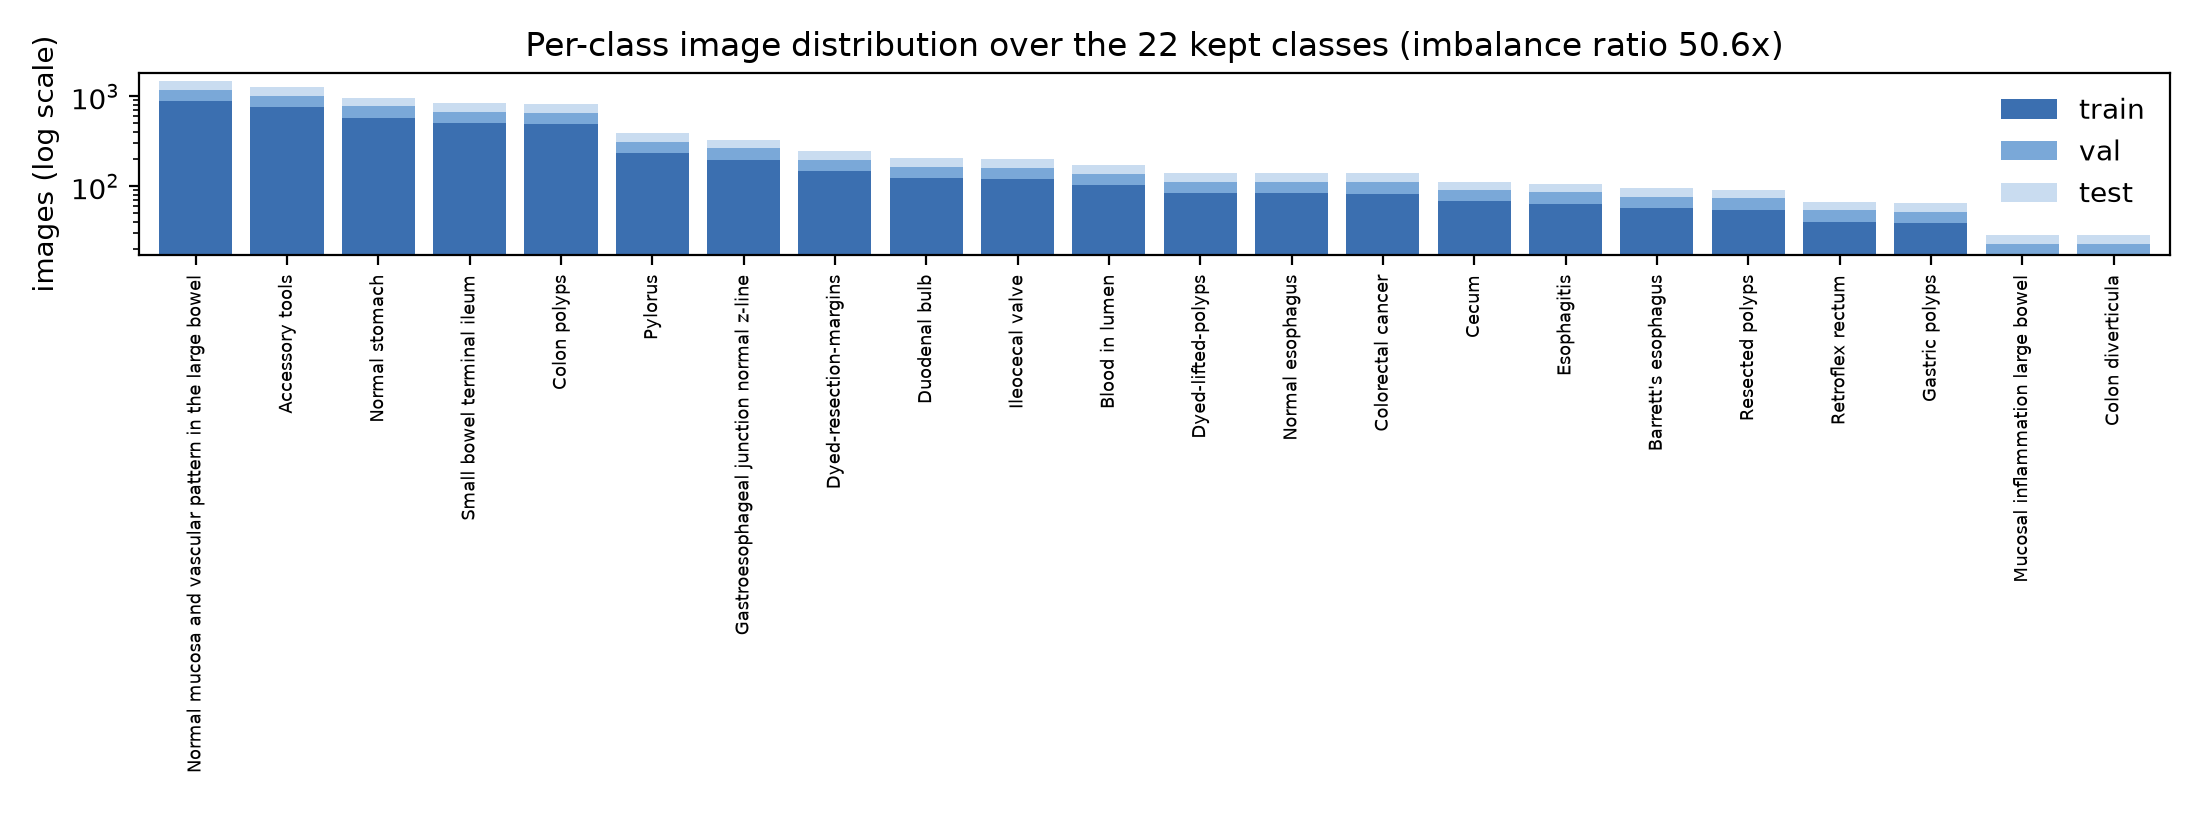
\includegraphics[width=\linewidth]{figures/fig_eda.png}
\caption{Per-class image distribution over the 22 kept classes
(stacked train/val/test, log scale). The imbalance ratio is $50.6\times$; two
classes (Mucosal inflammation large bowel, Colon diverticula) have only 6 test
images each.}
\label{fig:eda}
\end{figure}

\subsection{Reproducing the baseline honestly}
Under the paper's own rule --- best-by-validation checkpoint, no TTA --- our
DenseNet-121 gives $\mathbf{0.6686\pm0.0234}$ over three seeds:
$+0.0182$, i.e. $0.78\sigma$, in 30 epochs versus their 150. Three points must
be stated plainly, because this line supports the whole paper.
(i) We \emph{beat} the baseline here rather than matching it, and $\pm0.0234$ is
the largest standard deviation of any configuration in the study, dominated by a
single lucky seed. (ii) An earlier, independent run of the same
code\slash split\slash seed gave 0.6491, so \textbf{0.6504 lies between two of
our measurements} --- stronger
reproduction evidence than any single point estimate.
(iii) Since 0.6504 is a run without an error bar and our own DenseNet-121 spreads
$\pm0.0234$ across seeds, the honest reading is that 0.6504 carries an
unpublished uncertainty of at least $\pm0.02$; hence any ``we beat 0.6504'' must
rest on a CI excluding it.
The 30-epoch budget is fair to the baseline: DenseNet-121 peaks on validation at
epoch 6/30 (Sec.~\ref{sec:results}), so the remaining epochs could not have
helped it.

We do not release a split file (neither does the paper), but we \emph{verified}
our split against the paper's Table~3, which lists per-class test support:
16/22 classes match exactly, 6 differ by $\pm1$ image (rounding of a stratified
splitter), and the total is exactly 1{,}586. We therefore evaluate on a test set
of the same \emph{composition}, not merely the same size --- which later lets us
attribute the improvement class by class (Sec.~\ref{sec:perclass}).

\subsection{Integrity check 1: leakage and label noise}
Because multiple frames of one procedure are common in endoscopy, cross-split
leakage is the most serious integrity risk. Two checks over all 7{,}930 images:
an MD5 pass finds \textbf{one} byte-identical group crossing train/val (a Colon
polyps image; none touch the test set), and a near-duplicate pass
(cosine\,$\ge0.98$ on MobileNetV3-Small embeddings) finds \textbf{9 cross-split
pairs} affecting $6/1586=0.38\%$ of the test set. Removing those 6 test images
and recomputing changes \macroF{} by $\approx-0.002$ on every configuration
($-0.0016$ on the proposed model, a $1{:}59$ ratio against its $+0.0937$ gain):
leakage is not what produces the result, and this is now a measured statement.

The same scan returns something more valuable than leakage: near-identical
images carrying \emph{different} labels. Most striking, a \texttt{val/Esophagitis}
image and a \texttt{test/Normal esophagus} image are the same picture
(cosine $=1.0000$) under two clinically exclusive labels. This is a data-quality
ceiling: no model can be correct on both, and Esophagitis is indeed one of our
model's eight weakest classes (Sec.~\ref{sec:perclass}).

\subsection{Integrity check 2: determinism is per-GPU}
\label{sec:hw}
Before trusting any number we ran the same seed twice and compared the 3-epoch
validation trajectory. On A100 two runs agree to six digits
($[0.428608, 0.549646, 0.551532]$); the identical code on a T4 gives a
\emph{different} trajectory ($[0.430615, 0.540379, 0.541930]$); a later A100 run
reproduces the A100 trace exactly. \textbf{Determinism holds within a device,
not across devices}: same seed + same code + different GPU $=$ a different model.
The operational consequence is that a reported $\sigma$ must never mix hardware;
in this paper every configuration has all three seeds on the \emph{same} GPU
type (Tesla T4), so every $\sigma$ is clean.

An unplanned event turned this into a stronger measurement. When the project
moved infrastructure, four round-1 configurations were accidentally
\emph{retrained} on T4 rather than reloaded from stored logits, leaving a
complete replicate --- same code/split/seed, 4 configs $\times$ 3 seeds
$\times$ 6 scoring rules, on two GPU types (Table~\ref{tab:hw}). Three readings
follow, all of which enter the paper: (i) the hardware shift accumulates from
$\approx0.010$ at 3 epochs to $0.04$--$0.07$ after 30 epochs plus checkpoint
selection; (ii) the \texttt{top3} rule is $\approx4\times$ more hardware-robust
than any single-checkpoint rule; and (iii) \textbf{the round-1 architecture
ranking does not survive a change of GPU} --- under \texttt{top3\_tta}, A100
gives $P1>S0>P0>B0$ while T4 flips it to $B0>S0>P1>P0$. A ranking reversed by a
GPU swap is not a ranking, and this is independent evidence for the humility we
are forced into in Sec.~\ref{sec:archcmp}.

\begin{table}[t]
\centering
\caption{Unplanned A100$\leftrightarrow$T4 replicate: mean absolute
\macroF{} disagreement across 4 configurations (same code/split/seed), by
scoring rule. \texttt{top3} is the most hardware-robust rule.}
\label{tab:hw}
\begin{tabular}{lcc}
\toprule
Scoring rule & $|\overline{\Delta}|$ over 4 configs & max $|\Delta|$ at one seed \\
\midrule
\texttt{top3}       & \textbf{0.0046} & 0.0263 \\
\texttt{top3\_tta}  & 0.0092 & 0.0310 \\
\texttt{smooth}     & 0.0153 & 0.0710 \\
\texttt{best}       & 0.0182 & 0.0435 \\
\texttt{smooth\_tta}& 0.0185 & 0.0717 \\
\texttt{best\_tta}  & 0.0185 & 0.0428 \\
\bottomrule
\end{tabular}
\end{table}

%==============================================================================
\section{Models and Method}
\label{sec:methods}
%==============================================================================

\subsection{Three branches, one protocol}
We compare three ImageNet-1k pretrained backbones spanning the local--global
inductive-bias axis (Table~\ref{tab:models}). The reference baseline is
DenseNet-121 (CNN, local). We add Swin-T~\cite{swin} as a Transformer baseline
(global self-attention via windowed W-MSA/SW-MSA), which the original paper does
not include. The proposed backbone is CoAtNet-0~\cite{coatnet}, a published
hybrid with convolutional early stages (local inductive bias, data efficiency)
and attention in later stages (global layout).

We deliberately use the hybrid \emph{as published and fully pretrained} rather
than hand-assembling ``Swin-T + a conv stem'': freshly initialized conv layers
attached to a pretrained transformer would confound \emph{architecture} with
\emph{initialization quality}, exactly the failure mode that dominates on this
$\approx$8k-image dataset (Sec.~\ref{sec:transfer}). For the same reason all
three baselines use ImageNet-1k weights; swapping Swin-T to its stronger
ImageNet-22k weights would break the balance of the CNN-vs-Transformer
comparison, so that is held out as a separate ablation (Sec.~\ref{sec:perclass}).

\begin{table}[t]
\centering
\caption{The three backbones. All initialized from ImageNet-1k weights and
trained under one shared round-1 protocol (AdamW $10^{-4}$, 30 epochs, batch 32,
no per-branch tuning).}
\label{tab:models}
\begin{tabular}{lll r}
\toprule
Role & Model & Family & Params \\
\midrule
Reference baseline & DenseNet-121 & CNN (local) & 7.0\,M \\
New baseline & Swin-T & Transformer (global) & 27.5\,M \\
Proposed backbone & CoAtNet-0 & Hybrid (conv+attn) & 26.7\,M \\
\bottomrule
\end{tabular}
\end{table}

\subsection{Training recipes and the two-stage design}
Normalization uses ImageNet mean/std for all three backbones (a contract of the
pretrained weights, not a free choice). Three recipes are implemented:
\texttt{plain} (round-1: resize $\to$ horizontal flip $\to$ normalize),
\texttt{strong} (adds rotation, color-jitter, random-erasing --- measured and
discarded, see below), and \texttt{modern} (\texttt{plain} + light
RandAugment~\cite{randaugment} + mixup~\cite{mixup}, with cosine LR + 5-epoch
warmup + layer-wise LR decay 0.75 + EMA, over 80 epochs). Domain reasoning drives the augmentation choices: horizontal flip is
kept (no fixed mirror symmetry in the GI tract), while rotation (injects
interpolated black borders --- an endoscopy artifact), color-jitter (mucosal
color \emph{is} a diagnostic cue for Esophagitis, Barrett's, blood), and
random-erasing (many classes hinge on one small local structure) are rejected as
they corrupt the very signal that separates pathology from normal mucosa.

The proposed system stacks four elements on the CoAtNet-0 @288 backbone:
the \texttt{modern} recipe; a top-3 checkpoint ensemble (Sec.~\ref{sec:ckpt});
inference-time logit adjustment (Sec.~\ref{sec:logit}); and TTA-free scoring.
We name configurations for later reference:
\texttt{B0} (DenseNet-121 @224), \texttt{S0} (Swin-T @224),
\texttt{P0} (CoAtNet-0 @224), \texttt{P1} (CoAtNet-0 @288, \texttt{plain}),
\texttt{P2} (CoAtNet-0 @288, \texttt{modern}, \emph{reported system}),
\texttt{P2b} (DenseNet-121 @224, \texttt{modern}),
\texttt{P2c} (CoAtNet-0 @224, \texttt{modern}).

\subsection{Checkpoint selection: 0 epochs, universal, hardware-robust}
\label{sec:ckpt}
If validation is small and noisy, then picking one best-by-val checkpoint is a
\emph{noisy measurement}, not model selection. We keep multiple states in a
single training run so that one run yields six test numbers: three selectors
(\texttt{best} = raw val peak; \texttt{smooth} = peak of 3-epoch-smoothed val;
\texttt{top3} = logit ensemble of the three best-val checkpoints) $\times$
$\{$with, without horizontal-flip TTA$\}$. Ranking the six rules across the four
round-1 configurations (only those four vote, so that adding a later tier cannot
silently flip the reported rule), \texttt{top3} wins (mean rank 1.50 vs 2.00 for
\texttt{top3\_tta}). We therefore fix \texttt{SELECTION\_RULE = top3} for the
\emph{entire} paper --- one rule applied to every row, rather than the best rule
per model (which would be a leak). Moving \texttt{best}$\to$\texttt{top3} is
positive on all four architectures (mean $+0.0188$) and nearly halves variance
($\overline\sigma$ $0.0163\to0.0080$); combined with Table~\ref{tab:hw} it is
the cheapest way to make the \emph{other} measurements resolvable. Its value is
in the $\sigma$ column, not the $\Delta$ column: $+0.0188$ is itself below the
0.035 threshold.

\subsection{Logit adjustment}
\label{sec:logit}
Logit adjustment~\cite{logitadj} subtracts $\tau\cdot\log(\text{class prior})$
from the logits at inference, with $\tau$ tuned on validation:
\begin{equation}
\hat y = \arg\max_{c}\;\big[\, z_c - \tau\,\log \pi_c \,\big],\qquad
\pi_c=\frac{n_c}{\sum_{k}n_k},
\end{equation}
where $z_c$ is the raw logit for class $c$ and $\pi_c$ its training prior. It is
the only zero-GPU lever that targets the imbalance bias directly. The notebook
enforces a pre-registered accept/reject test: keep it only if it both raises the
mean and does not inflate $\sigma$ beyond $1.5\times$. On the proposed model it
passes cleanly ($+0.0143$, $\sigma$ \emph{shrinks} $0.0096\to0.0088$, stable
$\tau^\star\in[0.3,0.5]$); on the weaker \texttt{P1} it barely passes
($+0.0052$, below its own $\sigma$, one seed selecting $\tau^\star=0$).
Section~\ref{sec:discussion} returns to why this asymmetry is a methodological
lesson rather than a footnote.

%==============================================================================
\section{Results}
\label{sec:results}
%==============================================================================

\subsection{Architecture comparison: unresolvable at three seeds}
\label{sec:archcmp}
Table~\ref{tab:arch} gives \macroF{} over three seeds under \texttt{top3}, with
bootstrap 95\% CIs. The four round-1 configurations lie in $0.6780$--$0.6855$, a
spread of $0.0075$ that is \emph{smaller than their own $\sigma$}, and none has
a CI separated from 0.6504. The pre-registered decision rule --- ``if Swin-T
only ties DenseNet-121, the backbone-is-the-bottleneck hypothesis is not
supported'' --- fires: $S0-B0=+0.0033$ and $P0-B0=+0.0034$, both below $\sigma$,
with paired per-seed McNemar $p\approx0.50$. Combined with the GPU-swap ranking
reversal (Sec.~\ref{sec:hw}), the correct statement is that \textbf{the three
architectures are not separable on this test set} --- weaker, and truer, than
``they tie.''

\begin{table}[t]
\centering
\caption{Architecture comparison, \texttt{top3}, three seeds. Only
CoAtNet-0 + the modern recipe (\texttt{P2}, \texttt{P2c}) clears the bar of a CI
excluding 0.6504; the standalone architecture swap does not.}
\label{tab:arch}
\setlength{\tabcolsep}{4pt}
\begin{tabular}{l c c l}
\toprule
Config & \macroF{} (3 seeds) & vs.\ 0.6504 & bootstrap 95\% CI (seed 0) \\
\midrule
\texttt{B0} DenseNet-121 (CNN)      & $0.6780\pm0.0073$ & $+0.0276$ & $[0.6412,0.7239]$ n.s. \\
\texttt{S0} Swin-T (Transformer)    & $0.6813\pm0.0081$ & $+0.0309$ & $[0.6307,0.7167]$ n.s. \\
\texttt{P0} CoAtNet-0 @224 (Hybrid) & $0.6814\pm0.0100$ & $+0.0310$ & $[0.6229,0.7103]$ n.s. \\
\texttt{P1} CoAtNet-0 @288          & $0.6855\pm0.0068$ & $+0.0351$ & $[0.6364,0.7185]$ n.s. \\
\midrule
\textbf{\texttt{P2}} CoAtNet-0 @288 + modern & $\mathbf{0.7298\pm0.0096}$ & $\mathbf{+0.0794}$ & $\mathbf{[0.6660,0.7531]}$ \\
\texttt{P2c} CoAtNet-0 @224 + modern (1 seed) & $0.7172$ & $+0.0668$ & $[0.6664,0.7568]$ \\
\texttt{P2b} DenseNet-121 @224 + modern & $0.6670\pm0.0119$ & $+0.0166$ & $[0.6319,0.7227]$ n.s. \\
\bottomrule
\end{tabular}
\end{table}

\subsection{The gain decomposition and the \texorpdfstring{$2{\times}2$}{2x2} interaction}
\label{sec:decomp}
The proposed system wins by \emph{stacking independently measured levers}, not by
a mysterious new architecture. Table~\ref{tab:cumulative} closes the additive
path exactly ($0.7441-0.6686=+0.0755$), and Table~\ref{tab:decomp} restates it
as a decomposition against the resolvability threshold. One lever --- the modern
recipe --- accounts for 59\% of the gain and is the \emph{only} lever above
$\pm0.035$. The two levers the study was designed to test, architecture and
resolution, sum to $+0.0075$ (10\%) and sit inside the noise; the two
``measurement'' levers add $+0.0237$ (31\%) at zero extra epochs.

\begin{table}[t]
\centering
\caption{Cumulative path of the proposed system, all under \texttt{top3}. The
resolution step is measured under the \emph{old} recipe; under the modern recipe
it is $-0.0006$ (Sec.~\ref{sec:decomp}), so it describes the path taken, not a
transferable property.}
\label{tab:cumulative}
\begin{tabular}{l l c}
\toprule
Step & From $\to$ to & $\Delta$ \\
\midrule
Checkpoint rule & \texttt{B0} best $0.6686\to$ \texttt{B0} top3 $0.6780$ & $+0.0094$ \\
Architecture (CNN$\to$hybrid) & \texttt{B0} $0.6780\to$ \texttt{P0} $0.6814$ & $+0.0034$ \\
Resolution $224\to288$ & \texttt{P0} $0.6814\to$ \texttt{P1} $0.6855$ & $+0.0041$ \\
\textbf{Modern training recipe} & \texttt{P1} $0.6855\to$ \texttt{P2} $0.7298$ & $\mathbf{+0.0443}$ \\
Logit adjustment (0 epochs) & \texttt{P2} $0.7298\to 0.7441$ & $+0.0143$ \\
\midrule
& \textbf{total} & $\mathbf{+0.0755}$ \\
\bottomrule
\end{tabular}
\end{table}

\begin{table}[t]
\centering
\caption{Lever decomposition under one scoring rule. Only the modern recipe
clears the $\pm0.035$ resolvability threshold; architecture and resolution ---
the levers we set out to test --- are indistinguishable from zero.}
\label{tab:decomp}
\begin{tabular}{l c c}
\toprule
Lever & $\Delta$ \macroF{} & Clears $\pm0.035$? \\
\midrule
Modern training recipe (\texttt{P1}$\to$\texttt{P2}) & \textbf{+0.0443} & \textbf{yes} \\
Inference logit adjustment (0 epochs)                & $+0.0143$ & no \\
Checkpoint rule \texttt{best}$\to$\texttt{top3} (0 epochs) & $+0.0094$ & no \\
Resolution $224\to288$ (old recipe; new: $-0.0006$)  & $+0.0041$ & no \\
Architecture swap DenseNet$\to$CoAtNet (standalone)  & $+0.0034$ & no \\
\midrule
& \textbf{total $+0.0755$} & \\
\bottomrule
\end{tabular}
\end{table}

Because the modern recipe helps the hybrid but \emph{hurts} the CNN, it cannot
be a universal lever. The clean control \texttt{P2b} (DenseNet-121 @224 +
modern) gives $-0.0110$ over three seeds, 3/3 negative, and is lower even on
validation. A completed $2{\times}2$ design separates the two candidate causes.
On the same seed~0 (the tightest comparison, since \texttt{P2c} has one seed):
\begin{center}\small
\begin{tabular}{l c c c}
\toprule
@224, seed 0 & old recipe & modern recipe & $\Delta$ \\
\midrule
DenseNet-121 (CNN)   & 0.6878 & 0.6835 & $-0.0043$ \\
CoAtNet-0 (hybrid)   & 0.6718 & \textbf{0.7172} & $+0.0454$ \\
\bottomrule
\end{tabular}
\end{center}
Each factor \emph{alone} is $\le0$ (architecture $-0.0160$; recipe $-0.0043$),
while together they give $+0.0294$; the interaction term is
$0.0454-(-0.0043)=+0.0497$. Averaged over the full design, the
recipe\,$\times$\,architecture term is $\mathbf{+0.0468}$ (clears $\pm0.035$)
and recipe\,$\times$\,resolution is $+0.0085$ (does not) --- and both survive a
change of scoring rule. \textbf{The gain is an interaction between recipe and
architecture, not a sum of two levers}, which is precisely the structure a
$2{\times}2$ design reveals and two lone comparisons cannot.

This also overturns an implicit assumption of ours: \textbf{$288$px is not what
makes the difference}. Under the modern recipe, $288$ vs $224$ is $-0.0006$
while costing $1.70\times$ the compute per image (Sec.~\ref{sec:deploy}), so the
configuration that \emph{should be deployed} is \texttt{P2c} @224 --- the same
resolution as the baseline, cheaper, and not worse. We still \emph{report}
\texttt{P2} because it has three seeds and a known $\sigma$, while \texttt{P2c}
has one.

\paragraph{Beating both baselines.}
The assignment asks whether the proposed model beats \emph{both} baselines.
Pairing on the same test images: \texttt{P2} vs \texttt{B0} is
$+0.0430\,[+0.0147,+0.0691]$ (significant at 2/3 seeds), and \texttt{P2} vs the
Transformer baseline \texttt{S0} is $+0.0384\,[+0.0074,+0.0708]$ (significant at
3/3 seeds). The proposed model clears both.

\subsection{Per-class analysis: where the improvement lands}
\label{sec:perclass}
The proposed model (\texttt{P2}, seed 0) reaches accuracy (micro-F1) $=0.850$
(paper: 0.8203) and macro precision $=0.810$ vs macro recall $=0.690$. The
0.120 precision--recall gap is the most informative number: the model is
\emph{cautious} on rare classes --- usually right when it names one, but missing
many --- which for a screening system is the less desirable error direction, and
which is exactly the prior-shift bias logit adjustment corrects.

Because our test split matches the paper's composition, the improvement can be
attributed class by class against their Table~3 (Table~\ref{tab:perclass}).
\textbf{90.4\% of the improvement comes from the 15 rare classes}
($<50$ test images), where mean $\Delta$F1 is $+0.086$; the 7 common classes are
essentially saturated ($+0.020$, 9.6\%). Clinically this is the right place: the
rare classes here are pathology (Barrett's, esophagitis, gastric/resected
polyps), the saturated common classes are normal anatomy. Five classes still
\emph{lose} to the paper (total $-0.0172$, of which $-0.0097$ is a single
6-image class), so the reported $+0.0937$ is a conservative estimate measured
\emph{after} absorbing those losses.

\begin{table}[t]
\centering
\caption{Improvement attributed by class size against the paper's Table~3
(proposed model, seed 0). The gain is concentrated in the rare (pathology)
classes; the common (normal-anatomy) classes are saturated.}
\label{tab:perclass}
\begin{tabular}{l c c c}
\toprule
Group & \# classes & mean $\Delta$F1 & contribution to \macroF{} \\
\midrule
Rare ($<50$ test images)   & 15 & $+0.086$ & $+0.0585$ (90.4\%) \\
Common ($\ge50$ test images) & 7 & $+0.020$ & $+0.0062$ (9.6\%) \\
All 22 classes             & 22 & $+0.065$ & $+0.0647$ \\
\bottomrule
\end{tabular}
\end{table}

The eight weakest classes (F1 $0.286$--$0.636$) are all among the smallest
classes (17--83 training images each, vs 760--880 for strong classes; see the
bottom of Fig.~\ref{fig:perclass}, where the red rare classes cluster below the
macro-F1 line). The bottleneck is \emph{feature representation from tail data},
not the loss function --- a diagnosis confirmed independently below.

\begin{figure}[t]
\centering
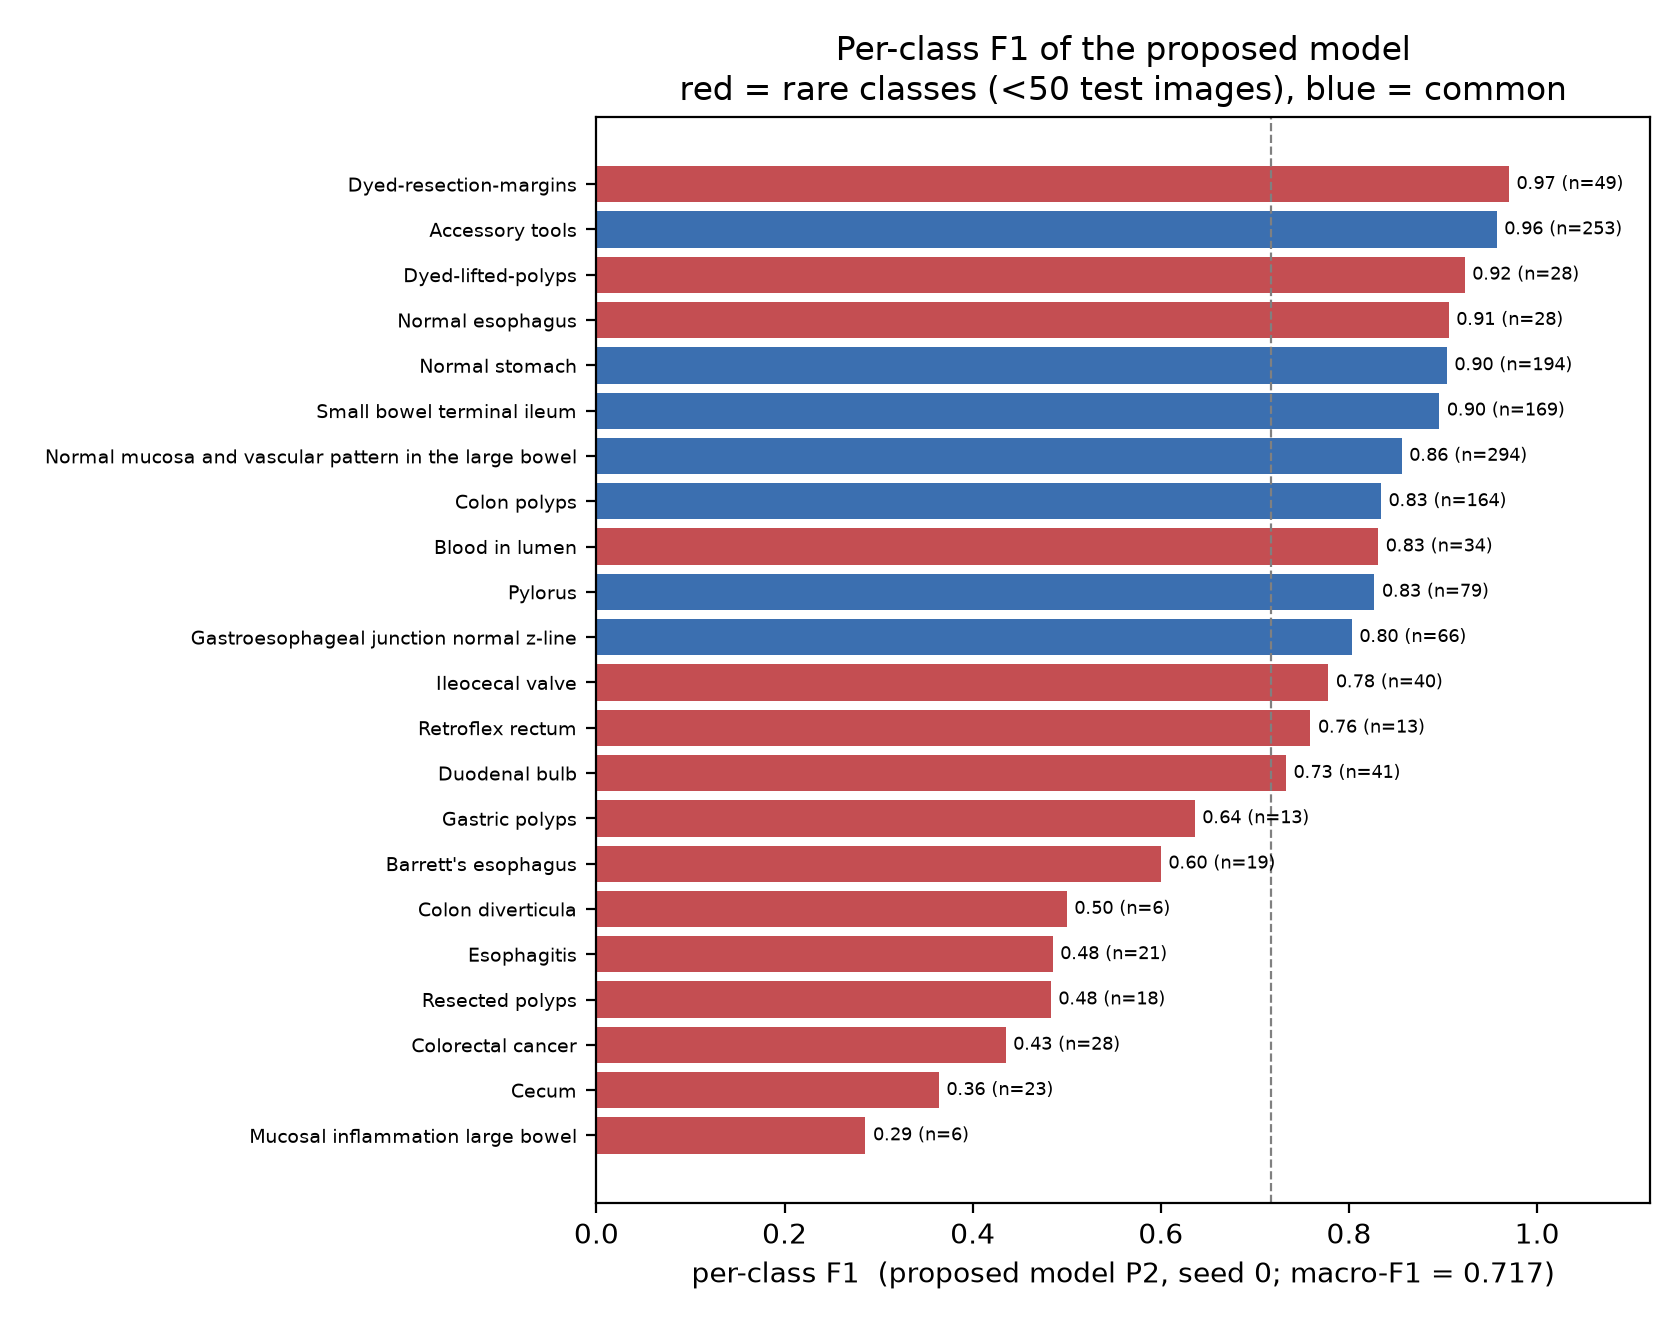
\includegraphics[width=0.82\linewidth]{figures/fig_perclass_f1.png}
\caption{Per-class F1 of the proposed model (\texttt{P2}, seed 0), sorted, with
test support $n$. Red = rare classes ($<50$ test images), blue = common; the
dashed line is the macro-F1 (0.717). Every class below the line is rare, which
is the per-class view of the ``bottleneck is tail data'' diagnosis.}
\label{fig:perclass}
\end{figure}

\paragraph{Training-time imbalance levers are flat; inference-time works.}
Three textbook long-tail levers applied \emph{at training time} do not move
\macroF{}: strong augmentation ($-0.035$), Balanced-Softmax~\cite{balms}
($-0.007$, and $-0.0047$ when re-measured under the current protocol --- a rare
\emph{reproducible} result, unfortunately of a negative), and decoupled
classifier retraining / cRT~\cite{decoupling} ($-0.013$). The cleanest comparison puts the two
approaches on the same backbone, seed, and epoch budget: on DenseNet-121 seed 0,
fixing imbalance \emph{in the loss} (Balanced-Softmax) gives $-0.0047$, while
fixing it \emph{at inference} (logit adjustment, $\tau^\star=0.4$) gives
$+0.0213$. Same target, two sites, opposite signs --- and the winning site costs
zero epochs. With $\approx17$ training images per tail class, re-weighting cannot
create information that is not there; shifting the decision boundary with one
validation-tuned parameter is cheap and effective.

\paragraph{Where the remaining headroom is.}
A ceiling analysis (set a group's F1 to 1.0 and read the resulting \macroF{})
shows that of the $0.2834$ remaining to the theoretical ceiling, \textbf{85.2\%
lies in the 15 rare classes} and only $+0.0420$ in \emph{all} 7 common classes
combined. Since a model-family lever must clear $\pm0.035$ to be provable, and a
\emph{perfect} model on the saturated common classes would gain only $+0.0420$,
\textbf{no further ``change the model'' lever can be demonstrated on this
1{,}586-image test set, regardless of GPU hours}. The remaining headroom is a
\emph{data} problem. A direct measurement supports this: changing only the Swin-T
pretraining weights from ImageNet-1k to ImageNet-22k buys $+0.0254$ --- more than
any architecture lever in the study, without changing a single architectural
line.

\subsection{Transfer learning: freeze vs.\ trainable}
\label{sec:transfer}
Four conditions on the \emph{same} DenseNet-121, same split/seed/budget, differ
only in trainable depth (Table~\ref{tab:transfer}). Full fine-tuning wins
decisively, and the cost of freezing rises steeply with depth: linear probing
gives away $-0.1106$ \macroF{} --- more than the entire $+0.094$ this project
gains over the published baseline. The reason: ImageNet features are
\emph{natural-image} features, while endoscopy is a different modality
(specular highlights, circular black masks, unnatural color statistics), so it
is precisely the \emph{early} layers that must move --- exactly what freezing
pins down. The paper corroborates this for free: its Table~2 mixes last-layer
tuning ($0.4496$--$0.4883$) and full fine-tuning ($0.6176$--$0.6504$), a $\sim0.16$
gap on this split. Since each frozen condition has one seed, we report only the
$>2\sigma$ gaps as real (T2 vs.\ T3 ordering is not).

\begin{table}[t]
\centering
\caption{Transfer learning on one DenseNet-121 (\texttt{top3}). Only trainable
depth varies. Full fine-tuning (= \texttt{B0}) wins; freezing the backbone ---
refusing to let features move --- is very costly.}
\label{tab:transfer}
\begin{tabular}{l l c c}
\toprule
Condition & What is trained & seeds & test \macroF{} \\
\midrule
T1 linear probe & classifier only & 1 & $0.5674$ \\
T2 freeze lower half & upper half + classifier & 1 & $0.6596$ \\
T3 progressive unfreeze + discriminative LR & probe$\to$full & 1 & $0.6394$ \\
T4 full fine-tune (= \texttt{B0}) & whole network & 3 & $\mathbf{0.6780\pm0.0073}$ \\
\bottomrule
\end{tabular}
\end{table}

\subsection{Learning curves and ensembles}
The two baselines finish learning early --- both peak on validation at
epoch 6/30 (Table~\ref{tab:curves}) --- confirming the 30-epoch budget is fair to
them. \texttt{P2} peaks at epoch 40/80 (half its budget) with a last-5-epoch
spread of $0.0019$, the smallest of all configurations: the fingerprint of EMA,
and the mechanical reason \texttt{P2} has a small $\sigma$ despite training
$\sim3\times$ longer. \texttt{P2b} peaks at $0.6539$ on validation --- below
\texttt{B0}'s $0.6600$ despite 80 epochs --- so the modern recipe fails
DenseNet-121 on validation as clearly as on test.

Two ensemble lines are reported separately because they spend several training
runs. A 3-seed ensemble of \texttt{P2} reaches $0.7587\,[0.7110,0.7924]$, the
project's highest number, at the cost of three trainings. A
multi-architecture ensemble selected on validation reaches only $0.7130$ ---
\emph{below} the best single model --- a negative result: averaging probabilities
dilutes a dominant member with weaker ones.

\begin{table}[t]
\centering
\caption{Validation learning summary. Both baselines peak at epoch 6/30 (the
30-epoch budget is generous); the proposed \texttt{P2} peaks at 40/80 with the
flattest EMA tail (last-5-epoch spread $0.0019$), while the modern recipe on
DenseNet (\texttt{P2b}) peaks \emph{below} the plain \texttt{B0} baseline.}
\label{tab:curves}
\begin{tabular}{l c c c}
\toprule
Config & best val \macroF{} & at epoch & last-5-epoch spread \\
\midrule
\texttt{B0} DenseNet-121        & 0.6600 & 6\,/\,30  & 0.0069 \\
\texttt{S0} Swin-T              & 0.6992 & 6\,/\,30  & 0.0178 \\
\texttt{P0} CoAtNet-0 @224      & 0.6653 & 19\,/\,30 & 0.0133 \\
\texttt{P1} CoAtNet-0 @288      & 0.6746 & 11\,/\,30 & 0.0290 \\
\textbf{\texttt{P2}} CoAtNet-0 @288 + modern & \textbf{0.7208} & 40\,/\,80 & \textbf{0.0019} \\
\texttt{P2b} DenseNet-121 + modern & 0.6539 & 19\,/\,80 & 0.0002 \\
\texttt{P2c} CoAtNet-0 @224 + modern & 0.7086 & 11\,/\,80 & 0.0018 \\
\bottomrule
\end{tabular}
\end{table}

%==============================================================================
\section{Deployment}
\label{sec:deploy}
%==============================================================================
All four models export to ONNX successfully. At batch 32 on T4, DenseNet-121 is
fastest ($3.18$ ms/image, matching its 7\,M parameters), CoAtNet-0 @224 is
$5.13$ ms and @288 is $8.74$ ms --- a $1.70\times$ resolution cost within the
$1.65\times$ pixel ratio, reproduced across two GPU types. The honest
cost/benefit statement: the proposed system buys $+0.0937$ \macroF{} at
$2.75\times$ compute per image, $3.9\times$ model size, and $5.5\times$ training
time, plus a $3\times$ inference factor for the top-3 checkpoint ensemble;
dropping to \texttt{P2c} @224 (only $-0.0006$ on seed 0) cuts the first factor
to $1.61\times$. A Gradio demo serves top-5 predictions with flip TTA and was
run end-to-end on a GPU-free machine (top-1 \emph{Accessory tools}, $p=0.961$).

An independent \textbf{CPU round} (15 epochs, batch 16, fp32, 3 seeds) confirms
the methodology on a third hardware type: it reproduces \texttt{top3} as the most
robust rule, reproduces the ``logit adjustment is flat without the modern
recipe'' finding, and issues its own pre-registered claim --- a 3-seed DenseNet
ensemble at $\macroF{}=0.7059\,[0.6560,0.7447]$, a CI that excludes 0.6504.
That is: \emph{even without a GPU, this pipeline beats the paper's published
number with confidence-interval evidence}. It is an independent claim on its own
protocol scale and is not merged with the T4 numbers.

%==============================================================================
\section{Discussion and Limitations}
\label{sec:discussion}
%==============================================================================
One methodological lesson appears three times, each from a different direction,
and is the paper's takeaway. (1) A four-architecture \emph{ranking} reverses
under a GPU swap (Sec.~\ref{sec:hw}). (2) The \emph{resolution lever} reads
$+0.0143$ on one hardware and $+0.0041$ on another (an earlier draft of this work
reported the former as ``the only effective data lever''). (3) The $\sigma$
itself --- the very ruler used to accept or reject levers --- was anomalously
small ($0.0016$) on one A100 run, which caused logit adjustment to be
\emph{wrongly discarded} in round 1 by the $1.5\times$-inflation test; the fix
was to re-measure the lever on the new model rather than inherit the old
conclusion, and that is exactly what rescued a $+0.0143$ effect. An effect
smaller than the replicate-to-replicate range of its own measurement is not an
effect.

We report the known limitations plainly. (i) The dominant uncertainty is
\emph{data}, not seeds: the bootstrap CI is $\pm0.035$ ($\sim3.6\times$ the seed
$\sigma$) because two of 22 classes have $<10$ test images, so buying more seeds
would not narrow it --- the right direction is few-shot or more tail data, which
is also the dataset authors' own recommendation. (ii) The strongest claim, the
recipe\,$\times$\,architecture interaction, currently rests on a one-seed cell
(\texttt{P2c}); raising it to three seeds is the most important missing
experiment ($\approx3.3$ T4-hours). (iii) The architecture comparison is
unresolvable at three seeds, so the local-vs-global motivation of
Sec.~\ref{sec:methods} remains a \emph{hypothesis}, not a measured conclusion.
(iv) The deployed demo is weaker than the reported system ($\texttt{best\_tta}$
$0.7199$ vs $0.7441$). (v) With no patient identifiers in the public release, a
patient-level split is infeasible from the public data; we substitute a two-layer
leakage audit and re-measure after removal, but the 9 pairs found are a lower
bound, not an upper one.

%==============================================================================
\section{Conclusion}
%==============================================================================
We beat the published GastroVision baseline --- $0.7441\pm0.0088$ vs $0.6504$,
with a 95\% CI excluding that number --- and the point of interest is
\emph{how}, because it is not how we intended. Decomposing the whole $+0.0755$
into independently measured levers, the two we designed the study to test ---
architecture ($+0.0034$) and resolution ($+0.0041$) --- sum to 10\% of the gain
and sit inside the noise; what pays is the training recipe ($+0.0443$, 59\%, the
only lever above the $\pm0.035$ threshold) and the measurement discipline
($+0.0237$, 31\%, at zero extra epochs). Even that is conditional: the same
recipe \emph{hurts} DenseNet-121 ($-0.0110$), and a completed $2{\times}2$
design attributes the gain to a recipe\,$\times$\,architecture interaction
($+0.0468$), not a lever that adds. The bottleneck is feature representation
from tail data, confirmed from four independent directions --- the eight weakest
classes are all among the smallest, 90.4\% of the improvement is in the 15 rare
classes, macro precision exceeds macro recall by 0.120, and freezing the
backbone costs 11.1 points --- so the remaining headroom is a data problem, not a
model one. If one sentence is to be carried away: \emph{on small medical
datasets, measure hard enough to be sure before trusting any lever --- because
most levers are smaller than the error of the measurement itself, and the one
that survives is not the one you set out to find}.

\paragraph{Reproducibility.} All numbers are extracted automatically from saved
notebook outputs (\texttt{extract.py}) or recomputed from stored logits
(\texttt{offline\_tables.py}); none are typed by hand. Models are implemented in
PyTorch with pretrained backbones from the timm library~\cite{timm}. Runs: Kaggle
Tesla T4, \texttt{SEEDS}$=[0,1,2]$, \texttt{SPLIT\_SEED}$=42$, AMP fp16; 30 epochs
for round-1 configurations and 80 epochs for the modern-recipe configurations.

%==============================================================================
\begin{thebibliography}{99}
\small
\bibitem{gastrovision} D.~Jha \emph{et al.}, ``GastroVision: A Multi-class
Endoscopy Image Dataset for Computer-Aided Gastrointestinal Disease Detection,''
\emph{ICML Workshop on Machine Learning for Multimodal Healthcare Data}, 2023.
arXiv:2307.08140.
\bibitem{kvasir} K.~Pogorelov \emph{et al.}, ``KVASIR: A Multi-Class Image
Dataset for Computer Aided Gastrointestinal Disease Detection,'' \emph{ACM
MMSys}, 2017.
\bibitem{hyperkvasir} H.~Borgli \emph{et al.}, ``HyperKvasir, a Comprehensive
Multi-class Image and Video Dataset for Gastrointestinal Endoscopy,''
\emph{Scientific Data}, vol.~7, no.~283, 2020.
\bibitem{resnet} K.~He, X.~Zhang, S.~Ren, and J.~Sun, ``Deep Residual Learning
for Image Recognition,'' \emph{CVPR}, 2016. arXiv:1512.03385.
\bibitem{densenet} G.~Huang, Z.~Liu, L.~van~der~Maaten, and K.~Q.~Weinberger,
``Densely Connected Convolutional Networks,'' \emph{CVPR}, 2017.
arXiv:1608.06993.
\bibitem{efficientnet} M.~Tan and Q.~V.~Le, ``EfficientNet: Rethinking Model
Scaling for Convolutional Neural Networks,'' \emph{ICML}, 2019. arXiv:1905.11946.
\bibitem{vit} A.~Dosovitskiy \emph{et al.}, ``An Image is Worth 16x16 Words:
Transformers for Image Recognition at Scale,'' \emph{ICLR}, 2021.
arXiv:2010.11929.
\bibitem{deit} H.~Touvron \emph{et al.}, ``Training Data-Efficient Image
Transformers \& Distillation Through Attention,'' \emph{ICML}, 2021.
arXiv:2012.12877.
\bibitem{swin} Z.~Liu \emph{et al.}, ``Swin Transformer: Hierarchical Vision
Transformer using Shifted Windows,'' \emph{ICCV}, 2021. arXiv:2103.14030.
\bibitem{coatnet} Z.~Dai, H.~Liu, Q.~V.~Le, and M.~Tan, ``CoAtNet: Marrying
Convolution and Attention for All Data Sizes,'' \emph{NeurIPS}, 2021.
arXiv:2106.04803.
\bibitem{convnext} Z.~Liu \emph{et al.}, ``A ConvNet for the 2020s,''
\emph{CVPR}, 2022. arXiv:2201.03545.
\bibitem{cbloss} Y.~Cui, M.~Jia, T.-Y.~Lin, Y.~Song, and S.~Belongie,
``Class-Balanced Loss Based on Effective Number of Samples,'' \emph{CVPR}, 2019.
arXiv:1901.05555.
\bibitem{balms} J.~Ren \emph{et al.}, ``Balanced Meta-Softmax for Long-Tailed
Visual Recognition,'' \emph{NeurIPS}, 2020. arXiv:2007.10740.
\bibitem{decoupling} B.~Kang \emph{et al.}, ``Decoupling Representation and
Classifier for Long-Tailed Recognition,'' \emph{ICLR}, 2020. arXiv:1910.09217.
\bibitem{logitadj} A.~K.~Menon \emph{et al.}, ``Long-tail Learning via Logit
Adjustment,'' \emph{ICLR}, 2021. arXiv:2007.07314.
\bibitem{mixup} H.~Zhang, M.~Cisse, Y.~N.~Dauphin, and D.~Lopez-Paz, ``mixup:
Beyond Empirical Risk Minimization,'' \emph{ICLR}, 2018. arXiv:1710.09412.
\bibitem{randaugment} E.~D.~Cubuk, B.~Zoph, J.~Shlens, and Q.~V.~Le,
``RandAugment: Practical Automated Data Augmentation with a Reduced Search
Space,'' \emph{NeurIPS}, 2020. arXiv:1909.13719.
\bibitem{seedvariance} D.~Picard, ``Torch.manual\_seed(3407) is All You Need,''
arXiv:2109.08203, 2021.
\bibitem{bootstrap} B.~Efron and R.~J.~Tibshirani, \emph{An Introduction to the
Bootstrap}. Chapman \& Hall/CRC, 1993.
\bibitem{timm} R.~Wightman, ``PyTorch Image Models (timm),''
\url{https://github.com/huggingface/pytorch-image-models}, 2019.
\end{thebibliography}

\end{document}
